% https://tex.stackexchange.com/questions/88949/curved-waved-lines-with-tikz
\documentclass[12pt,ngerman,parskip=half]{scrartcl}

\usepackage[utf8]{inputenc}
\usepackage[T1]{fontenc}
\usepackage[left=5mm,top=5mm,right=5mm,bottom=5mm]{geometry}
\usepackage{tikz}
\renewcommand{\familydefault}{\sfdefault}
\pagestyle{empty}

\begin{document}

\begin{tikzpicture}

\node[anchor=north west ,inner sep=0] (frame1) at (0,15)     {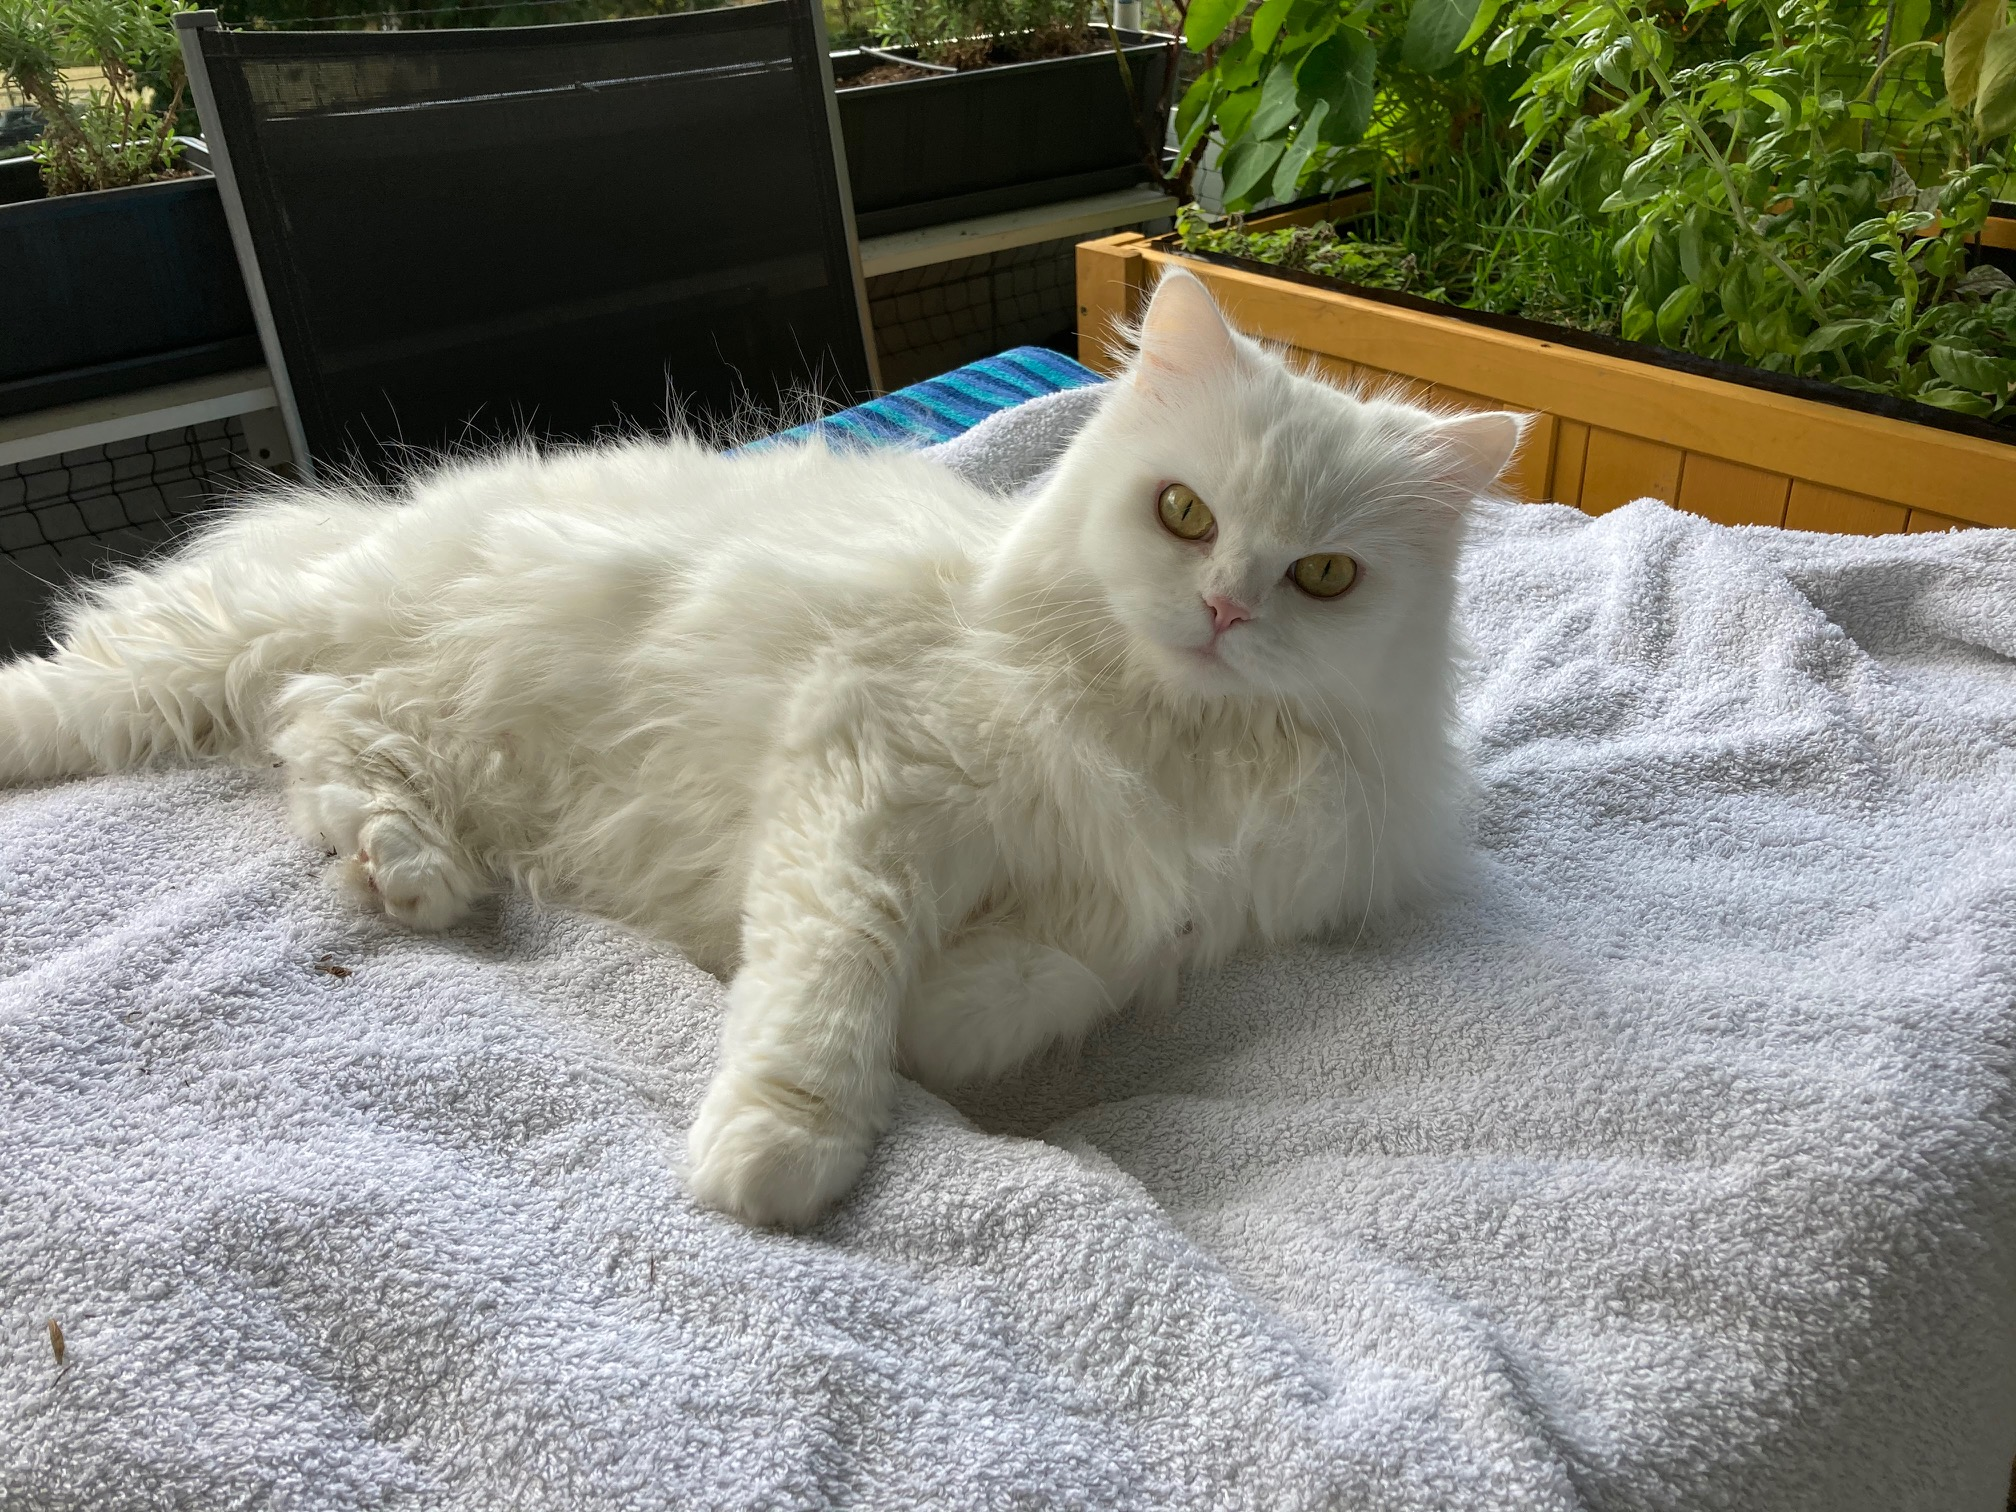
\includegraphics[width=19cm]{Katze1}};
\draw[help lines,red] (0,0) grid (20,15);
\foreach \xtick in {1,...,19} {\pgfmathsetmacro\result{\xtick} \node at (\xtick,-0.5) {\pgfmathprintnumber{\result}}; }
\foreach \ytick in {0,...,15} {\pgfmathsetmacro\result{\ytick} \node at (-0.25,\ytick) {\pgfmathprintnumber{\result}}; }

\node[rotate=-15] (ro) at (15,11.5) {\bfseries\Large\textcolor{yellow}{Ohr}};
\node[rotate=-15] (lo) at (11,13) {\bfseries\Large\textcolor{yellow}{Ohr}};
 
  
\end{tikzpicture}


\end{document}